\section{Gets and Multi-gets (90 pts)}

In this section, we measure the performance characteristics of the full system under mixed \texttt{GET-SET} workload. We experiment with 1, 3, 6, 9 keys for \texttt{get} requests, using memtier's \texttt{--multi-key-get=<Multi-Get size>} argument. 

Meanwhile, we control the workload ratio by \texttt{--ratio=1:<Multi-Get size>}, so each memtier client will send interleaving \texttt{set} and \texttt{get} requests one after another, so that the total numbers of keys in \texttt{set}s and in \texttt{get}s matches the specified ratio, while the total numbers of requests for each type are the same.

% For multi-GET workloads, use the \texttt{--ratio} parameter to specify the exact ratio between SETs and GETs. You will have to measure response time on the client as a function of multi-get size, with and without sharding on the middlewares.

\subsection{Sharded Case}

In this subsection, we run multi-gets with 1, 3, 6 and 9 keys with sharding enabled. The setup is listed in the table below. For this set of experiments, we choose 64 as the number of middleware worker threads, because it always provides the highest throughput in the system, as shown in Sections 3 and 4. Although in the previous sections when there are only 2 clients in each memtier instance, the throughputs were the same among different numbers of worker threads, in this section the large \texttt{multi-get} size may possibly put higher pressure on the workers, so it is also a safe choice to have 64 worker threads.

\begin{center}
	\scriptsize{
		\begin{tabular}{|l|c|}
			\hline Number of servers                & 3                       \\ 
			\hline Number of client machines        & 3                       \\ 
			\hline Instances of memtier per machine & 2                       \\ 
			\hline Threads per memtier instance     & 1                       \\
			\hline Virtual clients per thread       & 2     		            \\ 
			\hline Workload                         & ratio=1:$<$Multi-Get size$>$             \\
			\hline Multi-Get behavior               & Sharded                 \\
			\hline Multi-Get size                   & [1, 3, 6, 9]                  \\
			\hline Number of middlewares            & 2                       \\
			\hline Worker threads per middleware    & 64 \\
			\hline Repetitions                      & 3 $\times$ 80 seconds each     \\ 
			\hline 
		\end{tabular}
	} 
\end{center}

Figure~\ref{fig:5.1_responsetime} is the response time measured by memtier on its average, as well as 25\textsuperscript{th}, 50\textsuperscript{th}, 75\textsuperscript{th}, 90\textsuperscript{th} and 99\textsuperscript{th} percentile, with regard to multi-get size. The average response times fit the interactive law, both on the middleware side (with RTT added as think time) and on the memtier side.

\begin{figure}[!h]
\parbox{.5\linewidth}{
\centering
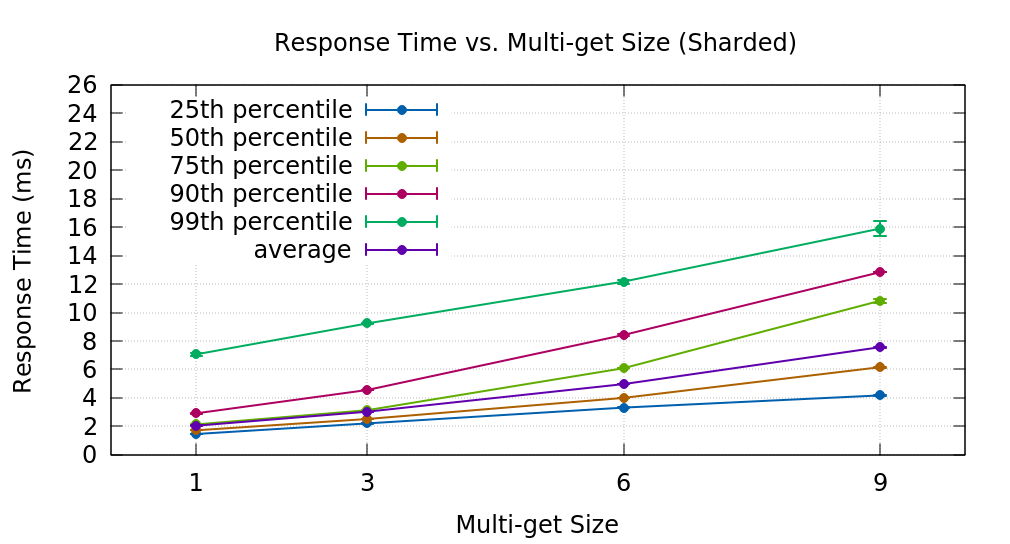
\includegraphics[width=0.5\textwidth]{img/5_1_responsetime.png}
\captionsetup{justification=centering}
\caption{\label{fig:5.1_responsetime}Memtier Response Time (Sharded)\\(Error bars are too small to be distinguished)}
}
\parbox{.5\linewidth}{
\centering
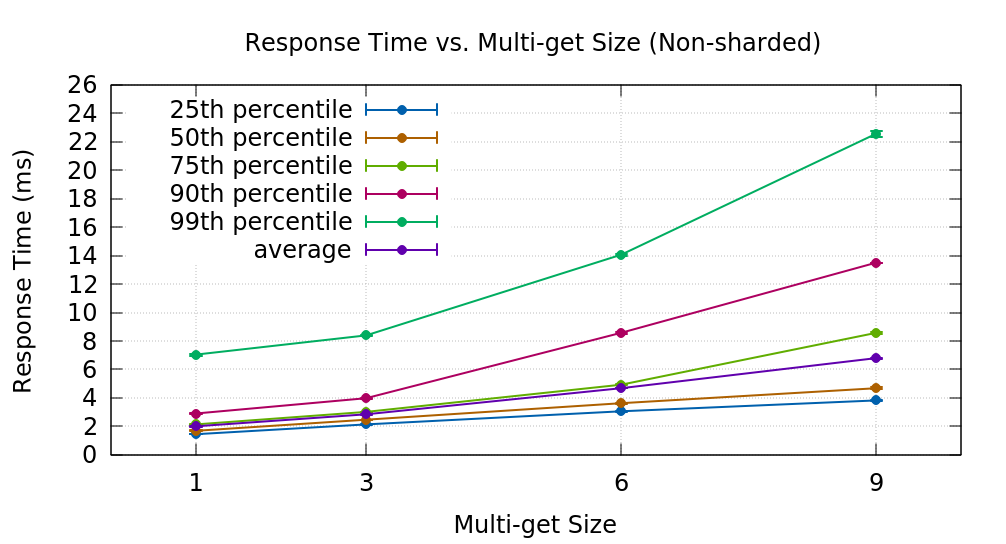
\includegraphics[width=0.5\textwidth]{img/5_2_responsetime.png}
\captionsetup{justification=centering}
\caption{\label{fig:5.2_responsetime}Memtier Response Time (Non-sharded)\\(Error bars are too small to be distinguished)}
}
% \end{figure}

% \begin{figure}[!h]
\centering
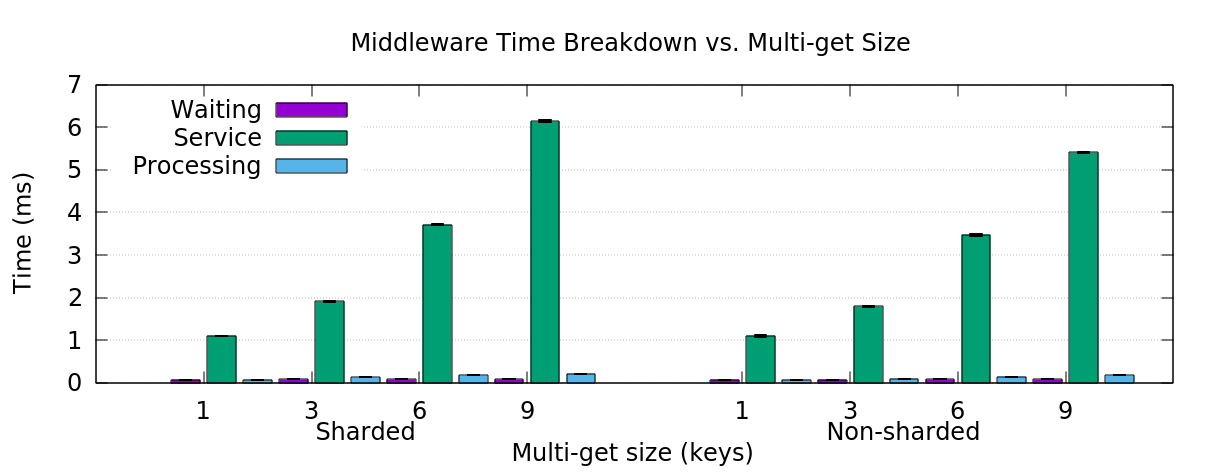
\includegraphics[width=0.8\textwidth]{img/5_breakdown.png}
\captionsetup{justification=centering}
\caption{\label{fig:5_breakdown}Middleware Time Breakdown (Sharded vs Non-sharded)\\(Error bars are too small to be seen clearly)}
\end{figure}

\subsubsection{Explanation}

% Provide a detailed analysis of the results (e.g., bottleneck analysis, component utilizations, average queue lengths, system saturation). Add any additional figures and experiments that help you illustrate your point and support your claims.

From the response time plots we can see that for every percentile (and the average), the response time always grows with multi-get size, which is reasonable because the more keys would require more service time. This is indeed supported by Figure~\ref{fig:5_breakdown}, left part: the memcached service time for 6-key and 9-key multi-gets is respectively about two and three times that of 3-key multi-gets. Note that although for 1-key and 3-key gets, the middleware always sends 1-key gets to servers, the average service time of 3-key is still larger than 1-key, because for 1-key gets, each request is sent to one server with uniform distribution, so the finally aggregated average service time is the average of three servers, while for 3-key gets, each request is split into three, one 1-key get is sent to each server and the middleware waits for all three responses, so the average service time is determined by the slowest server's service time, plus some parsing overhead (the request processor is implemented in such a way that it will parse the response in the mean time of receiving it). 

The \texttt{get} (\texttt{multi-get}) throughputs in 1,3,6,9-key experiments are 2705.54 ops/sec, 2181.43 ops/sec, 1445.69 ops/sec and 986.36 ops/sec respectively, or
2705.54 keys/sec, 6544.29 keys/sec, 8674.14 keys/sec and 8877.24 keys/sec respectively, as measured by memtier. Middleware measurements are very close, within 1\% error bound. For 1 and 3 keys, the bottleneck is the small number of clients, because no component is observed as saturated. For 6 and 9 keys, however, the bottleneck is again at the sending bandwidth of memcached servers, because this many keys per second (plus the additional \texttt{set} responses) have required the servers to send at a total bandwidth of 36 MiB/s. The servers' \texttt{dstat} logs indeed support this claim. 9-key experiments have resulted slightly more keys per second than 6-key, because the ratio of \texttt{set}s and \texttt{get}s is $1:1$, so 9-key experiments have less \texttt{set}s involved, leaving more traffic available for \texttt{get}s. The middleware is never a bottleneck, and consistently, our middleware logs show that the average queue length and the queue-waiting time has always been about zero.


\subsection{Non-sharded Case}

In this subsection, we run multi-gets with 1, 3, 6 and 9 keys with sharding disabled. As the maximum throughput is always reached by 64 worker threads, and also for the purpose of controlling variates, we still choose 64 as the number of worker threads.

\begin{center}
	\scriptsize{
		\begin{tabular}{|l|c|}
			\hline Number of servers                & 3                       \\ 
			\hline Number of client machines        & 3                       \\ 
			\hline Instances of memtier per machine & 2                       \\ 
			\hline Threads per memtier instance     & 1                       \\
			\hline Virtual clients per thread       & 2                		 \\ 
			\hline Workload                         & ratio=1:$<$Multi-Get size$>$              \\
			\hline Multi-Get behavior               & Non-Sharded             \\
			\hline Multi-Get size                   & [1, 3, 6, 9]                  \\
			\hline Number of middlewares            & 2                       \\
			\hline Worker threads per middleware    & 64 \\
			\hline Repetitions                      & 3 $\times$ 80 seconds each      \\ 
			\hline 
		\end{tabular}
	} 
\end{center}
%% say Figure 5.2 "at last page"?
Figure~\ref{fig:5.2_responsetime} is the response time measured by memtier on its average, as well as 25\textsuperscript{th}, 50\textsuperscript{th}, 75\textsuperscript{th}, 90\textsuperscript{th} and 99\textsuperscript{th} percentile, with regard to multi-get size. The average response times fit the interactive law, both on the middleware side (with RTT added as think time) and on the memtier side.

\subsubsection{Explanation}

% Provide a detailed analysis of the results (e.g., bottleneck analysis, component utilizations, average queue lengths, system saturation). Add any additional figures and experiments that help you illustrate your point and support your claims.
Similar to the sharded case, the average response time, as well as the percentiles of different levels, grows with regard to the number of keys, as shown in Figure~\ref{fig:5.2_responsetime}. Further, we can conclude from Figure~\ref{fig:5_breakdown} that the growth is mostly due to the increase in memcached service time, and the memcached service time for 6-key and 9-key multi-gets is respectively about two and three times that of 3-key multi-gets. However, for one-key get, the service time is 63.5\% of the 3-key case (instead of only $\frac{1}{3}$), because it is dominated by the network latency.

% bottleneck analysis

The bottlenecks are also the same as in the sharded case. For 1-key and 3-key \texttt{get}s, the throughput (measured by memtier; middleware measurements are within 1\% error bound, similarly hereinafter) is 2754.25 ops/sec and 2230.97 ops/sec respectively, which is only limited by the low number of clients. For 6-key and 9-key \texttt{get}s, the throughput is 1464.44 ops/sec and 993.21 ops/sec respectively, or 8786.64 keys/sec and 8938.89 keys/sec, with the overhead of \texttt{set} requests added, both has reached the sending bandwidth limit of memcached servers, which can also be proved from the \texttt{dstat} logs of three servers, so the bottleneck is again the server bandwidth. The middleware never becomes a bottleneck and gets saturated, as the queue waiting time and average queue length are always close to zero.


\subsection{Histogram}

\begin{figure}[!h]
\parbox{.5\linewidth}{
\centering
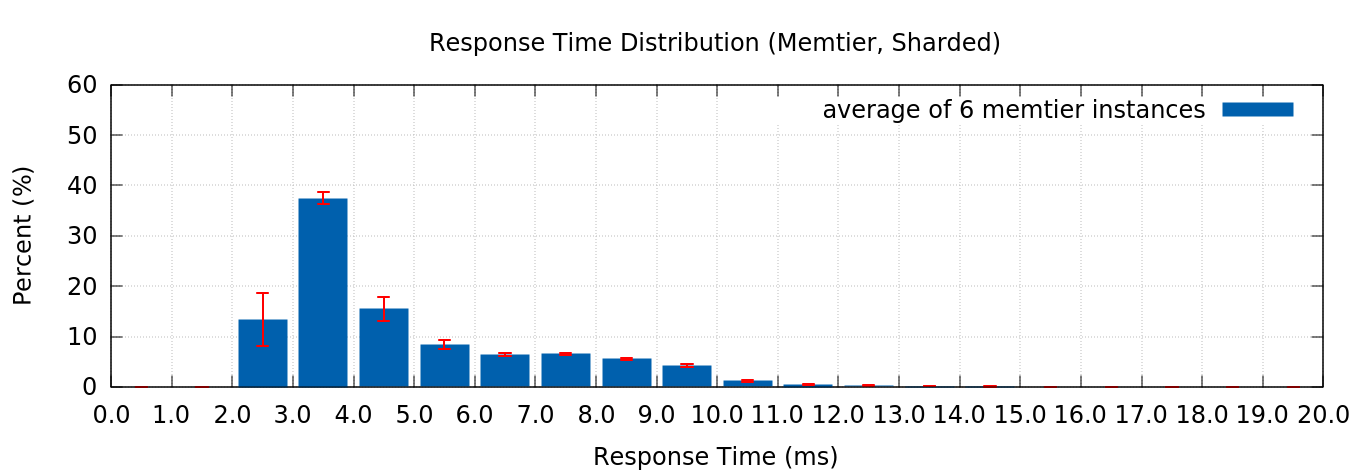
\includegraphics[width=0.5\textwidth]{img/5_1_histogram_client.png}
\captionsetup{justification=centering}
\caption{\label{fig:5.1_histogram_client}Memtier Histogram (Sharded)}
}
\parbox{.5\linewidth}{
\centering
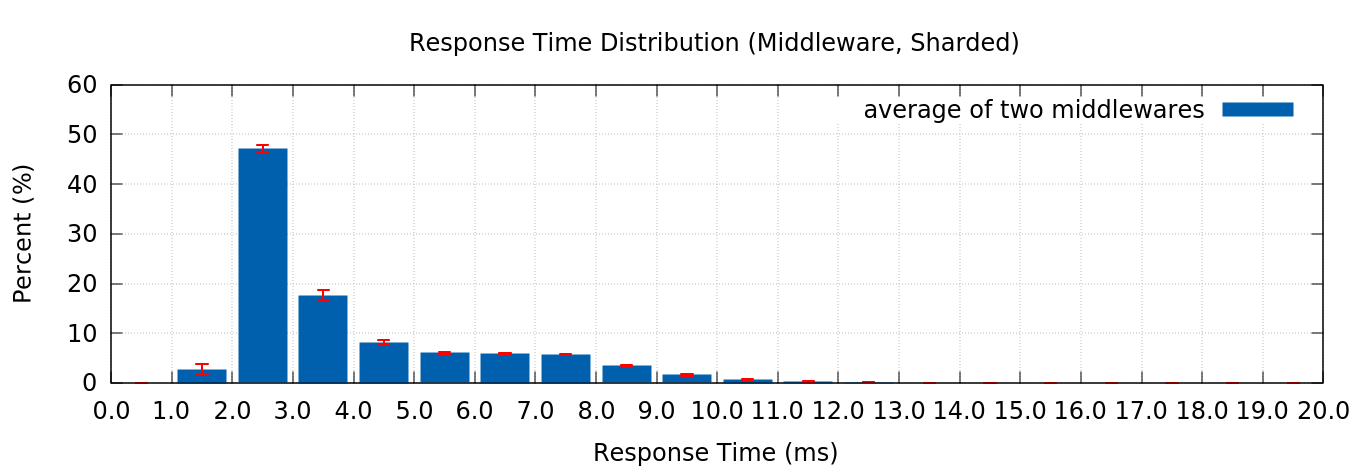
\includegraphics[width=0.5\textwidth]{img/5_1_histogram_mw.png}
\captionsetup{justification=centering}
\caption{\label{fig:5.1_histogram_mw}Middleware Histogram (Sharded)}
}
% \end{figure}

% \begin{figure}[!h]
\parbox{.5\linewidth}{
\centering
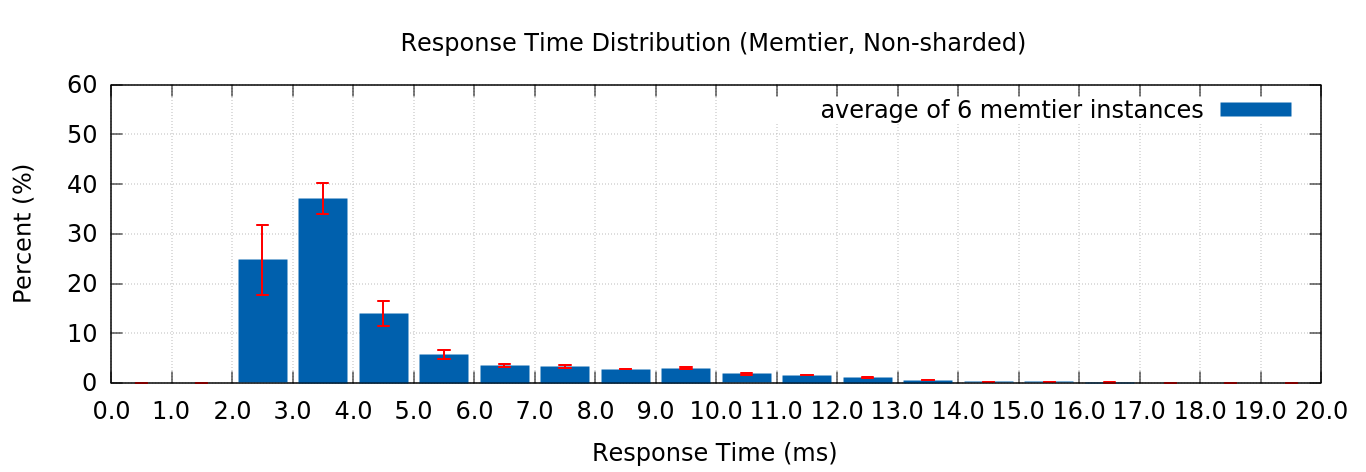
\includegraphics[width=0.5\textwidth]{img/5_2_histogram_client.png}
\captionsetup{justification=centering}
\caption{\label{fig:5.2_histogram_client}Memtier Histogram (Non-sharded)}
}
\parbox{.5\linewidth}{
\centering
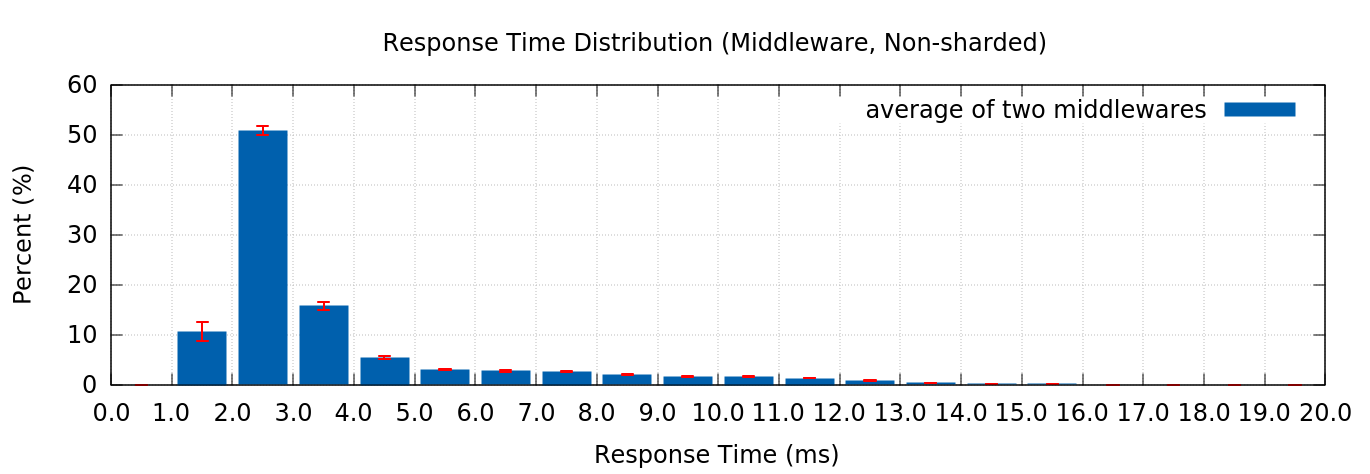
\includegraphics[width=0.5\textwidth]{img/5_2_histogram_mw.png}
\captionsetup{justification=centering}
\caption{\label{fig:5.2_histogram_mw}Middleware Histogram (Non-sharded)}
}
\end{figure}

Figures~\ref{fig:5.1_histogram_client} $\sim$ \ref{fig:5.2_histogram_mw} are four histograms for the case of 6-key-\texttt{multiget}s representing the sharded and non-sharded response time distribution, both as measured on the client, and inside the middleware. Every histogram has a bucket size of one millisecond, and twenty buckets in total. Due to the long-tail effect because the server is sometimes a little bit unstable, there are rare instances of requests whose response time is higher than 20.0 ms, but such requests are fewer than 0.2\% of the population, so they can be safely ignored.

The first observation is that the response time distribution has a long tail, with a majority hit in $2.0 \sim 5.0$ ms (memtier side) and a maximum hit at 14 ms for non-sharded 12 ms for sharded. The long tail effect is less significant in the sharded case than in non-sharded, because utilizing all three servers mitigates the randomness of the service time of a single server, making the overall response time more stable and the distribution more focused below 10 ms. This conclusion could also be drawn from the response time comparisons (Figures~\ref{fig:5.1_responsetime} and~\ref{fig:5.2_responsetime}): the 99\textsuperscript{th} percentile response time of sharded case is significantly lower than non-sharded.

Also worth noting is that the distribution measured by the middleware is entirely 1 ms lower than on memtier, and the $2.0 \sim 3.0$ bucket holds significantly more requests than the $1.0 \sim 2.0$ bucket. The main reason is that the network latency between clients and middlewares, which is on average 1 ms as well, is not included in the middleware measurements. Also, the network latency is also fairly unstable, with a mean standard deviation of 0.72 ms, so the response time difference is rather variable round 1 ms, making the middleware histogram not strictly 1-ms-shifted from the other side. 

\subsection{Summary}

% Provide a detailed comparison of the sharded and non-shareded modes. For which multi-GET size is sharding the preferred option? Provide a detailed analysis of your system. Add any additional figures and experiments that help you illustrate your point and support your claims.

The table below lists our performance measurements with standard deviations in brackets.

\begin{table}[!ht]
\centering
\resizebox{\linewidth}{!}{%
\begin{tabular}{|l|l|l|l|l|l|l|}
\hline
\multirow{2}{*}{Keys} & \multicolumn{2}{l|}{Throughput (ops/sec)} & \multicolumn{2}{l|}{Throughput (keys/sec)} & \multicolumn{2}{l|}{Mean Response Time (ms)} \\ \cline{2-7} 
                                       & Sharded           & Non-sharded       & Sharded            & Non-sharded           & Sharded             & Non-sharded            \\ \hline
1                                      & 2705.54 (35.76)   & 2754.25  (34.97)  & 2705.54 (35.76)    & 2754.25  (34.97)      & 2.05  (0.03)        & 2.01   (0.02)          \\ \hline
3                                      & 2181.43 (8.97)    & 2230.97  (16.71)  & 6544.29 (26.91)    & 6692.91  (50.13)      & 3.03  (0.01)        & 2.85   (0.01)          \\ \hline
6                                      & 1445.69 (0.18)    & 1464.44  (2.19)   & 8674.14 (1.08)     & 8786.64  (13.14)      & 4.97  (0.01)        & 4.68   (0.01)          \\ \hline
9                                      & 986.36  (0.83)    & 993.21   (0.97)   & 8877.24 (7.47)     & 8938.89  (8.73)       & 7.56  (0.03)        & 6.80   (0.03)          \\ \hline
\end{tabular} %
}
\end{table}


From the table we can see clearly that sharding multi-key \texttt{get}s and distributing the shards to all servers always makes the response time slightly larger than simply relaying the original request to one server, despite that the request size has been reduced. For 1-key \texttt{get}s, whether sharding is enabled makes no difference because single-key \texttt{get}s are always processed by the same function in the middleware implementation, so the throughput and response time keeps the same (within reasonable experimental error bound). For 3-, 6- and 9-key \texttt{multi-get}s, Figure~\ref{fig:5_breakdown} shows that the memcached service time with sharding enabled is slightly higher than the non-sharded case. This is understandable because in the \texttt{ShardedRequestProcessor} of the middleware, receiving from all three servers is implemented in a synchronous way, i.e. there is a loop to receive from the servers one by one, so overhead of receiving from two more servers, as well as the response-assembling overhead, could override the the time saved by smaller number of keys, especially when there exists a server whose network RTT with the middleware is considerably higher than others, this server will be a drag in the whole process. The middleware processing time for sharding is also slightly larger, because new requests need to be assembled before being sent to servers, and this part is not counted into the memcached service time.

Comparing the response time means and percentiles, we find despite that the mean, 25\textsuperscript{th}, 50\textsuperscript{th} and 75\textsuperscript{th} percentile response time of non-sharded is always lower than sharded, however, for the 99\textsuperscript{th} percentile, response time for sharded of any \texttt{multi-get} size is lower than non-sharded, because as explained already, performing sharding to utilize all three servers with less keys for each server could potentially reduce the randomness of multi-key service time of simply sending all keys to one server, thus mitigating the long-tail effect.

Finally, the response time histograms from memtier and middleware all feature a peak around $2.0 \sim 5.0$ ms, while middleware response time is entirely lower than memtier by about 1 ms, because it does not include the communication latency between memtier and middleware. For throughputs, for 1- and 3-key the maximum throughput is limited by the number of clients, as no component is found to be fully utilized; for 6-key and 9-key the system do hit the maximum throughput limited by the servers' sending bandwidth. This bottleneck analysis applies for both sharded and non-sharded. Although the throughput numbers for non-sharded experiments are slightly higher than sharded (taking standard deviations into account), the differences are actually very small, because the overhead introduced to the middlewares and the workload reduced for the servers are very close to each other. However, we do observe that as we increase the \texttt{multi-get} size, the sharded throughput becomes closer to non-sharded, so we do have a reason to believe that for even larger sizes of \texttt{multi-get}s, sharding may become a better option because the dominating part in the response time would be each server's service time, instead of the synchronised network communication overhead and request/response assembling overhead, thus the decrease on service time for larger sizes will make more sense.

In summary, in our system, for 1-,3-,6-,9-key \texttt{multi-get}s, sharding is never a better option because of the processing and network communication overhead introduced cannot be hidden by the reduced request size.